\section{Comparació exploratòria DDPG--TD3}\label{sec:ddpg}

\begin{figure}[htbp]
  \centering
  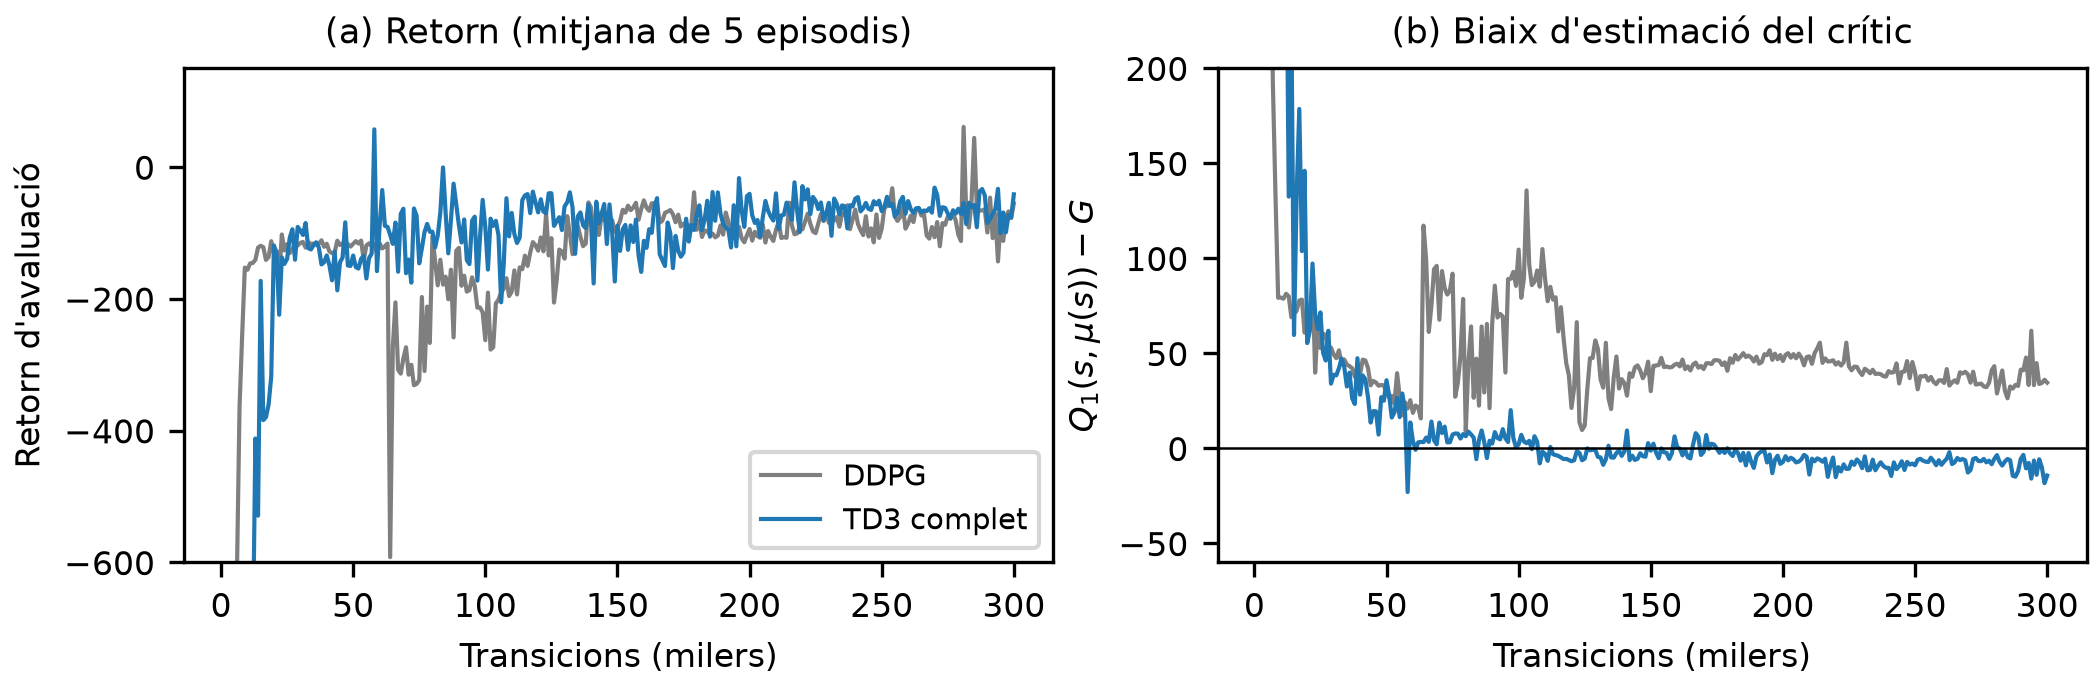
\includegraphics[width=\linewidth]{img/fig_ddpg_td3.png}
  \caption{Comparació exploratòria amb la llavor 0. (a) Retorn d'avaluació, mitjana de 5 episodis deterministes cada 1.000 transicions; l'eix vertical està retallat a −600 (els valors inicials són d'uns −1.440). (b) Biaix $Q_1(s,\mu(s))-G$ als episodis d'avaluació.}
  \label{fig:ddpg}
\end{figure}

A la Figura~\ref{fig:ddpg}, totes dues execucions surten del retorn inicial d'uns −1.440 en poques avaluacions (DDPG supera −200 als 9.000 passos i TD3 als 15.000) i acaben en un nivell semblant: L10 de −83,6 per a DDPG i de −70,3 per a TD3. La diferència clara és al crític: al final, el de DDPG sobreestima el retorn en 40,2 punts de mitjana, mentre que el primer crític de TD3 queda lleugerament per sota ($-10{,}6$), que és la direcció que motiva TD3 \parencite{fujimoto2018}. Amb una sola llavor per algorisme i dos sorolls d'exploració diferents, aquesta comparació no és evidència d'una diferència de rendiment.
